\documentclass[conference,final]{IEEEtran}

\usepackage{graphicx}
% \usepackage{epsfig}
\usepackage{subfigure}
\usepackage[hypertex]{hyperref}
\usepackage{subfigure}  
\usepackage{color}
\usepackage{pdfsync}
% \usepackage{draftcopy}

\usepackage[small,it]{caption}

\usepackage{multirow}
\usepackage{ifpdf}

\long\def\comment#1{{ \bf \textcolor{magenta}{\bf #1}}}
\long\def\ccomment#1{{ \bf \textcolor{blue}{\bf #1 (SJ)}}}
\newcommand{\F}[1]{\B{\textcolor{red}{FIXME: #1}}}
\newcommand{\C}{\comment}
\newcommand{\CC}{\ccomment}
\newcommand{\fix}[1]{\textcolor{red}{\bf #1}}
\newcommand{\tc}{$T_c$}

\newif\ifdraft
\drafttrue

\ifdraft
\newcommand{\fixme}[1]{ { \bf{ ***FIXME: #1 }} }
\newcommand{\jhanote}[1]{ {\textcolor{red} { ***Jha: #1 }}}
\newcommand{\yyenote}[1]{ {\textcolor{blue} { ***yye00: #1 }}}
\else
\newcommand{\jhanote}[1]{}
\newcommand{\yyenote}[1]{}
\newcommand{\fixme}[1]{}
\fi

\newcommand{\jitter}[1]{{$\sigma(\alpha)$}}

\newif\ifpdf
\ifx\pdfoutput\undefined
  \pdffalse
\else
  \ifnum\pdfoutput=1
    \pdftrue
  \else
    \pdffalse
  \fi
\fi

\ifpdf
\DeclareGraphicsExtensions{.pdf, .jpg}
\else
\DeclareGraphicsExtensions{.eps}
\fi

\begin{document}

\title{\large Developing Autonomic Distributed Scientific
  Applications: A Case Study From History Matching Using Ensemble
  Kalman-Filters}
  
\author{\authorblockN{Yaakoub El Khamra\authorrefmark{3}\authorrefmark{1}, Shantenu Jha\authorrefmark{1}\authorrefmark{2}},
   \authorblockA{\authorrefmark{1}
    Center for Computation and Technology, Louisiana State University,
    Baton Rouge, 70803} \authorblockA{\authorrefmark{2} Department of
    Computer Science, Louisiana State University, Baton Rouge, 70803}
    \authorblockA{\authorrefmark{3} Texas Advanced Computing Center, 
    University of Texas, Austin, 78758}
}
\maketitle
 \begin{abstract}
   The development of simple, effective distributed applications
   remains challenging.  Therefore, not surprisingly, it is difficult
   to implement advanced application characteristics -- such as
   autonomic behaviour. However, there exist a large class of
   applications which could benefit immensely with support for
   autonomic properties.  For example, many applications have
   irregular execution characteristics and highly variable resource
   requirements which are very difficult to predict in advance, but
   can be addressed using autonomic approaches.  Autonomics can help
   meet this promise. This paper discusses the design and development
   of a prototype framework using SAGA -- aptly called Lazarus, that
   can support many of the requirements of Autonomic applications that
   desire to use Computational Grids.  The development of such
   applications is difficult, but so is the effective deployment of
   such applications on Grids.  For example, as a consequence of
   irregular execution characteristics dynamic resource requirements
   are difficult to predict a priori thus rendering static resource
   mapping techniques such as workflows ineffective.  We provide here
   an initial description of the features and the architecture of the
   Lazarus framework, integrate it with an Ensemble Kalman Filter
   application, and demonstrate the advantages -- performance and
   lower development cost of the Lazarus framework.  As proof of
   concept we deploy Lazarus on several different machines on the
   TeraGrid, and show the effective utilization of several
   heterogeneous resources and distinct performance enhancements.
 \end{abstract}
 \begin{keywords}
   eScience Application, Middleware Inter-operation, Distributed
   Infrastructure Deployment, Distributed Application Programming,
   Cactus, Performance, SAGA, Programming Abstractions, Batch Queue
   Prediction BQP
 \end{keywords}

\section*{Notes}

To deal with the increasing complexity of large-scale computing
systems, computers and applications must learn to manage themselves in
accordance with high-level guidance from humans -- a vision that has
been referred to as autonomic computing.  Grids have the following
properties: (i) faulty, error-prone, (ii) dynamic resources, and (iii)
heterogeneous. But not all characteristics -- autonomic or otherwise,
have to be coded against.  Abstractions, such as frameworks to
facilitate reuse.  Application-level information that can than be
translated, for example, a policy or a strategy.. Present SAGA as a
programming system to develop Autonomic Application.  Provides
generalized, extensible mechanisms for:
\begin{itemize}
\item  Resource Selection
\item Placement
\item  Fault Tolerance -- what are we going to say? Manual implementation
\item Ability to plug-into decision support and Information Services
  systems
\item in general a framework can relieve the pressure/onus off the
  application developer for a wide range of application
\end{itemize}

And we apply this to an application that is a "prototypical"
application

\begin{itemize} 
\item Dynamic requirement
\item Highly-irregular and  difficult to plan/predict
\begin{itemize} 
  \item number of jobs
  \item distribution of the size of jobs
  \item time to completion between stages
\end{itemize} 
\item checkpoint and self-migrating 
\item Need for performance 
\end{itemize} 

In this paper we discuss:
\begin{itemize} 
\item Details of: Application Requirement $\rightarrow$ Resource Properties 
$\rightarrow$ Resource Selection
\item Performance Measures:
  \begin{itemize}
\item Define a workload and the time to complete 
\item Define a time and the number of jobs completed (throughput)
\item Scalability (number of systems utilized)
\end{itemize} 
\end{itemize} 



\section{Introduction}

% \jhanote{Reference Manish's earlier work on accord and reservoir simulations}
% \yyenote{So I added a small sentence there, do you want more?}

By definition Grids are characterized as dynamic and heterogeneous
environments.  They are dynamic due to time-dependent resources loads,
availability and access patterns; the aggregation of specialized
resources in different administrative domains is one source of the
heterogeneity.  Most tools to address the dynamical nature of the
grids assume a fixed underlying resource requirement.  There exist
several well known examples of distributed applications which in turn
have multiple 'embarrassingly' distributed jobs (or sub-applications)
that are either typically uncoupled or the coupling is between the
master and client application.  Things get significantly more
complicated when there is horizontal coupling between the distributed
jobs, say for example, a global exchange or synchronization point.
Most applications and support-tools for distributed applications
assume that the individual ``jobs'' during the course of their run
life-time will display a well-defined, static execution
characteristics.  However there are class of applications for which
the individual job run time characteristics are inherently difficult
to predict and plan for.  In addition to the class of applications we
investigate here -- Kalman filters~\cite{DataAssim, KalmanPaper},
there are ``first principles'' Grid applications such as
GridSAT~\cite{gridsat03} and applications which based upon resource
aware ``learning'' algorithms~\cite{ majority_voting}, for which it is
both difficult to estimate precisely the resource requirements while
explicitly needing to marshal the distributed resources . For these
applications the resource requirement is dynamic and unpredictable;
interestingly, the resource requirements and utilization might
possibly be dependent upon both the execution trajectory and
underlying infrastructure. Such applications are hard to develop and
deploy, but surprisingly, they have traditionally not received the
same level of infrastructural support for the development. It is
difficult to define a scheduling strategy that will be effective
throughout the execution of a complete applications; hence static
resource mapping is not an option.  It can be argued that the logic
for adapting to resource requirement changes from within the
application are best addressed at the application level.

% \yyenote{Feel free to move this, this is what I want to say about
%   Manish} \jhanote{this is perfect. thanks. its both technically
%   correct and strategically good} 
This certainly is not the first time autonomic frameworks have been
used to launch and manage reservoir simulations. Bangerth et al
\cite{Manish} used an autonomic framework to manage reservoir
simulations for well-placement optimization. At the moment, our work
is focused on history matching and reservoir characterization, however
the next logical step is to adapt Lazarus to run well/perforation
placement studies. This might lead to a convergence of SAGA and
Accord~\cite{accord} in terms of common functionality through
different approach.

\jhanote{needs to be shortened} A key impediment to accelerated
development of Grid applications and consequently the uptake of Grids
is the scarcity of high-level application programming abstractions
that bridge the gap between existing grid middle-ware and
application-level needs.  Application developers are daunted by the
complexity of the vast array of low-level Grid and distributed
computing software APIs that currently exist; APIs have traditionally
been developed using a bottom-up approach that exposes the broadest
possible functionality.  Coding using these bottom-up APIs requires
extremely verbose code to implement even the simplest of
application-level capabilities.  Many Grid computing
projects~\cite{gat, cog, realitygrid} recognized the need for
higher-level programming abstractions to simplify the use of
distributed computing for application developers.  The Simple API for
Grid Applications (SAGA) attempts to consolidate community effort and
make ends meet by employing a top-down approach to distributed
computing software infrastructure.  SAGA is the first comprehensive
attempt to provide a programmatic approach for the development of
applications so as to utilize distributed environments, either by
design or by virtue of deployment.  In addition to simplifying the
programming environment for application developers, SAGA insulates
applications from technological, version changes and other low-level
implementation details that regularly occur in the lower layers of the
software stack.

HPC Grid projects such as TeraGrid and DEISA have definitely provided
a massive increase in the computing power available for scientific
applications, but this is due to the individual parts, and nothing to
do with the sum of the parts, i.e., not because applications are able
to use distributed resources in a coupled or coordinated manner. The
ability of applications to scale-out -- a critical requirement for
distributed applications, has not been adequately developed or
supported. It has had limited success in engendering novel
applications or usage modes.


\jhanote{Refresh aim! This is GMAC @ ICAC!}  The aim of this paper is
to provide a rare example of a novel approach of developing
(programming) an application that can utilize the individual resources
of the TeraGrid in a coupled and coordination fashion, and not just a
single piece of big-iron.  We have captured the primary run-time
characteristics of an interesting and common class of applications and
implemented a solution to effectively manage this run-time complexity
at the {\it application level}.  Our solution is perfectly acceptable
as a proof-of-concept, and modulo deployment and resource availability
issues, our approach will scale to problem sizes encountered in the
many science and engineering problems with hard-to-predict run-time
characteristics.

% Grid Computing -- and its hollow (? -- at least so far) promise of
% providing unlimited computational capacity. Well the unlimited was
% always impractical -- but any attempts to scale-out have been almost
% ignored -- but the need has not. Thus applications  have had to resort
% to application-level solutions .... now introduce SAGA, abstractions,
% and all that jazz..

% Admittedly, the e size of our input problem that we use is small, and
% thus makes it unlikely to solve a problem of any real {\it scientific
%   impact} %to the petroleum and energy industry,
% however, 

% tools and support infrastructure to support and plan for resource
% variability have been developed.

% {\it mention the need for programmatic approach versus a grid
%   meta scheduler such as grid way or GR MS. mention that workflows are
%   good for static workloads. this in a way is a autonomic dynamic
%   application..}

% Grid way and other meta schedulers are designed to be able to account
% for dynamic resource characteristics -- fluctuations in availability,
% performance, load or proximity.


% {\it mention that these techniques are useful for first principles applications}
% {\it will need to reference AppLeS: application level scheduling
%   paper~\cite{apples03}}
%Mention what AppLeS does \& doesn't and why this work is different

% Applications that are designed for dynamic and heterogeneous
% environments require the ability to manage varying levels of
% heterogeneity and dynamical resources. 


\noindent The highlights of this paper are:

\noindent {\it Utilize the advantages of proper programming
  abstractions, by integrating SAGA and Cactus and demonstrate the
  usefulness for Grid application development:}
Cactus provides the support and features required to implement
adaptivity e.g., checkpoint, restart and migrate thorns. SAGA provides
the ability to implement these features in a specific distributed
environment, for example, move files from location A to location B,
start a job on resource X from resource Y.  Thus the two programming
abstractions that Cactus and SAGA provide are natural complements of
each other.  As alluded to, we do so by interfacing SAGA with Cactus
and thus are able to draw on the many advantages of using SAGA
function calls from within a Cactus application.  The result is an
application that uses these two important application-level frameworks
and abstractions to create a truly distributed application.  SAGA
provides the capability for the the distributed aspects. SAGA provides
a high-level programming interface to Grid functionality, and thus
presents arguably, for the first time ever, the ability to develop
complete and sophisticated applications using simple Grid function
calls.  This paper demonstrates the utility of SAGA for creating
applications that can perform across dynamic and heterogeneous
infrastructure.  Importantly, although we focus on a prototype of a
specific application -- Kalman filtering -- thanks to the architecture
and abstractions used, similar functionality can be trivially
incorporated in more sophisticated and complex applications.

\noindent {\it The development of an application that is adaptive in
  multiple ways:}
A working definition of adaptive applications can be given as
following: an application that can respond to a change in the run-time
environment and manage internally (ie without external user or control
intervention) the associated change of state and control-flow arising
from the change(s) in the run-time environment.  For some
applications, adaptivity as defined here would be an {\it interesting}
feature to have, ie., arguably of academic interest. As we will show,
for applications that have irregular run-time characteristics,
adaptivity is a {\it critical} feature, ie., a necessity.  For
example, once a model of application (as a job) has been mapped to a
resource, it is likely that the same model will have to be mapped to
another resource before the model reaches the desired convergence.
Thus for such applications , it is difficult to statically
(re-)schedule or manually control the execution of the jobs through
the application life-time.

Adaptivity may arise due to the number of processors required by the
many jobs being a variable, as well as the fact that the number of
stages (ie involving global synchronization and subsequent
distribution) is unknown {\it a priori}. There comes a point when
providing the mechanism (logic and control) to the applications
themselves to respond to these changes becomes more efficient and
reliable than leaving it to a scheduler (or a meta-scheduler for that
matter). We believe that this prototype application is well beyond the
transition point and is a classic example of an adaptive application.

The ability of a Cactus application to migrate to a more appropriate
resources based upon network characteristics was demonstrated in
Ref~\cite{escience07}.  We extend the sophistication of adaptivity to
include: migration to better resource, based upon both compute and
network characteristics, and choosing optimal resources to spawn to
based upon local queue characteristics (as well as compute and network
performance). The correct abstractions and programming approach
enables the simple codification of an application that can determine
best resource to migrate to based upon all of the above.

The outline of the paper is as follows: In the next section we outline
the scientific motivation and then describe the details of the
components of the application that we have developed to use SAGA and
Cactus.  \jhanote{to finish..}

\section{Application: Description and Motivation} 


\subsection{Ensemble Kalman Filters}


The specific application that we investigate -- a prototype
implementation of a ensemble Kalman filter using SAGA and Cactus -- is
a particularly interesting case of 'irregular, hard-to-predict run
time characteristics'.  The model needs to run to completion which is
defined as convergence to within a certain value.  The run time of
each model was unpredictable and uncorrelated with the run-time of
models running on the same number of processors -- a truly
independent variable.  As at every stage, each model must converge to
within a specified value before the next stage can begin, hence
dynamically load-balancing so as to ensure that all models complete as
close to each other as possible is the desired aim.  The number of
stages that will be required is not determined a priori. In the
general case the number of jobs required varies between stages.
Figure 1 shows a schematic of the irregular and hard to predict run
time characteristics of the simulations.

\jhanote{Place Appropriately...}

Even for relatively small input problem sizes at each stage, up to
several hundred models are generated which require from one to sixteen
processors to solve efficiently; the distribution of the number of
jobs and the run time-to-completion for a given processor count varies
by up to an order of magnitude.  Such hard to predict run-time
characteristics render static, data-flow independent scheduling
techniques difficult to use.  We demonstrate how the use of
appropriate programming abstractions like SAGA and Cactus enable the
effective development of applications with non-trivial requirements,
e.g., run-time resource selection based upon the application specific
characteristics.


% Modern reservoir simulators  Reservoir flow modeling
% exists in the context of of the reservoir management function, a
% process that optimizes the interaction between data and decision
% making during the life cycle of a field.  One of the more popular
% popular models is the model that is used to solve for the
%Ensemble Parallel Kalman filters can be used for solving
%multi-component, multi-phase flow of fluids~\cite{AzizSettari, },
%atmospheric modelling~\cite{yaakoub_reference_add} and a whole other
%range of scientific and engineering
%problems~\cite{yaakoubreferenceadd}.  Typical input to such
%simulations of multi-phase flow in porous geometry consists of the
%initial conditions of both fluids (saturation, temperature, pressure,
%density etc.) as well environmental conditions (porosity,
%permeability, depth etc.)

%To ensure the fidelity of the such simulations for real models, data
%from simulations is validated against experimental data. This process
%is referred to as history matching. In this process, a large number of
%simulations with different parameters or initial data, are run and
%their results fitted against the experimental data. When simulation
%results vary from experimental data, the input parameters are modified
%to bring the model closer to the real experimental data. This process
%is repeated until a consistency criteria is observerd. The fitting
%method can be anything from a genetic algorithm, an ensemble Kalman
%filter or a simulated annealing process.  Each has its merits and
%drawbacks.  One of the best methods to perform such convergence
%criteria is the ensemble Kalman~\cite{needreferencehere} filter
%method, and it requires a hard synchronization point where it gathers
%all the data from all the various models and modifies model parameters
%to get better history matching in the iterations to follow.

% Typical reservoir simulations can vary in size from 100 grid points to
% tens of millions of grid points, and a decent model space can contain
% upwards of hundreds of models each with possibly varying size,
% physical model (i.e equations to solve) and more importantly different
% rock and fluid properties.  

Ensemble Kalman filters (EnKF) are widely used in science and
engineering~\cite{DataAssim, KalmanPaper}. EnKF are recursive filters
that can be used to handle large, noisy data; the data can be the
results and parameters of ensembles of models that are sent through
the Kalman filter to obtain the true state of the data. The variation
in model parameters often has a direct and sizable influence on the
complexity of solving the underlying equations, thus varying the
required runtime of different models (thus the availability of the
results).  Varying parameters sometimes also lead to varying systems
of equations and entirely new scenarios. This obviously increases the
computational size requirements as well as memory requirements.  For
example as a consequence of the variation in size the underlying
matrix might become too large or even effectively doubling the number
of the system of equations, which could more than doubles the memory
required to solve the system of equations.
%Variation in non-linear terms in non-linear
%partial differential equations might also change the method used
%to solve the system of equations, which would vary the runtime as well
%as memory cost.

Hence a mechanism to assign models to available resources based on
their expected time to completion and resource requirement is useful.
Such a mechanism would estimate the time a model will spend in the
queue of a resource, the time it needs to run, and the time required
to migrate the data it requires/produces back and forth, and based on
that attempt to minimize the time required to perform each history
matching iteration.  In fact, with changing resource simulation
requirements (as is the case with models that find themselves lagging
behind the rest of the model pack), a mechanism which can take
advantage of of faster, cheaper or more powerful machines is even more
advantageous ~\cite{escience07}.

\begin{figure}
\begin{center}
\includegraphics*[scale=0.36,]{./figures/3StageKalmanFilter}
\end{center}
\caption{Schematic illustrating the irregular execution or
  hard-to-predict run-time characteristics of a prototype
  implementation of an ensemble kalman filter. The end-to-end
  application consists of several stages; in general at each stage the
  number of models generated varies. In the specific case studied in
  this paper, the size and granularity of the models varied within a
  stage. Consequently for any given stage the resource requirements
  varied from 8 processors to 64 processors.  The run time of each
  model was unpredictable and uncorrelated with the run-time of models
  on running on the same number of processors -- a truly independent
  variable. At every stage, each model must converge to within a
  specified value before the next stage can begin, hence dynamically
  load-balancing so as to ensure that all models complete as close to
  each other as possible is the desired aim.}
\label{fig:irregular_execution}
\end{figure}

\subsection{Programming Systems and Abstractions}

\jhanote{I think this section ought to be: i)SAGA ii) bigjob and iii) BQP }

... Our application
consists of a exemplary distributed simulation that uses the added
SAGA functionality to dynamically determine its ideal migration target
based on ad-hoc and statistical network characteristics and to migrate
itself in a heterogeneous Grid environment.  Although this a model
application it can be easily adapted to more complex scientific
applications.  Furthermore, our model application can be used as an
autonomous benchmarking agent for Grid resources. In this section we
briefly describe SAGA and the Cactus framework and discuss our
motivation to use SAGA to incorporate high-level Grid functionality
into Cactus.

\subsubsection{SAGA}

The Simple API for Grid Applications (SAGA) is an API standardization
effort within the Open Grid Forum (OGF)~\cite{ogf_web} an
international standards development body concerned primarily with
standards for distributed computing.  SAGA provides a simple,
POSIX-style API to the most common Grid functions at a sufficiently
high-level of abstraction so as to be able to be independent of the
diverse and dynamic Grid environments. The SAGA specification defines
interfaces for the most common Grid-programming functions grouped as a
set of functional packages.

\begin{itemize}
\item File package - provides methods for accessing local and remote
  filesystems, browsing directories, moving, copying, and deleting
  files, setting access permissions, as well as zero-copy reading and
  writing
\item Replica package - provides methods for replica management such
  as browsing logical filesystems, moving, copying, deleting logical
  entries, adding and removing physical files from a logical file
  entry, and search logical files based on attribute sets.
\item Job package - provides methods for describing, submitting,
  monitoring, and controlling local and remote jobs. Many parts of
  this package were derived from the largely adopted
  DRMAA~\cite{drmaa_url} specification.
\item Stream package - provides methods for authenticated local and
  remote socket connections with hooks to support authorization and
  encryption schemes.
\item RPC package - is an implementation of the GGF GridRPC
  API~\cite{gridrpc_url} definition and provides methods for unified
  remote procedure calls.
\end{itemize}

The two critical aspects of SAGA are its {\it simplicity} of use and
the fact that it is well on the road to becoming a community {\it
  standard}.  It is important to note, that these two properties are
provide the added value of using SAGA for Grid application
development.  Simplicity arises from being able to limit the scope to
only the most common and important grid-functionality required by
applications.  There a major advantages arising from its simplicity
and imminent standardization.  Standardization represents the fact
that the interface is derived from a wide-range of applications using
a collaborative approach and the output of which is endorsed by the
broader community.

The SAGA C++ reference implementation~\cite{saga_web} was incorporated
into the Cactus Code Framework in Ref~\cite{escience07} to provide the
needed Grid programming functionality.  We believe this was an
important step in merging two programming abstractions to achieve an
effect that is greater that sum of the parts. 

% The SAGA C++ reference implementation is being developed in close
% conjunction with the OGF standard.  Advert-service package which will
% most-likely be incorporated into a future version of the OGF standard.
% The SAGA C++ reference implementation comprise a complete set of local
% adaptors, an SQlite3 and PostgreSQL advert-service adaptor, and Globus
% pre-WS adaptors for file (GridFTP) and job (GRAM2) packages. We will
% go onto show how the application uses these features.

% \subsubsection{The Cactus Code~\cite{cactus_web}}
% Cactus~\cite{X0} is a framework for high performance scientific
% computing designed for scientists and engineers to develop and run
% codes for solving complex problems.  Developing code for high
% performance parallel machines has many challenges including
% scalability, efficiency (for computation, communication and
% input/output), portability and flexibility. Frameworks such as Cactus
% allow scientists and engineers to develop modules which can then be
% used together with modules written by other researchers to solve
% complex computational problems. The framework provides tools ranging
% from basic computational building blocks to complete toolkits that can
% be used to solve complex problems in astrophysics, computational fluid
% dynamics or other disciplines.  Tools developed in the Cactus Code
% framework run on a wide range of architectures including desktop PC's,
% supercomputers and computational Grids. Cactus and its associated
% toolkits are publicly available for download from the Cactus Code
% website.

% From an architectural standpoint, the Cactus Code framework consists
% of a central part (the ``flesh") and code modules (``thorns").  The
% flesh serves as a module manager, scheduling the routines of the
% thorns and passing data between thorns.  Thorns perform tasks ranging
% from setting up the computational grid, decomposing the computational
% grid for parallel processing, providing boundary and initial
% conditions.


%, communication of data from one processor to another,
%solving partial differential equations to input and output and
%visualization streaming. There are code modules that provide
%simulation control tools, such as the HTTPD thorn that sets up a web
%server for the simulation and allows researchers to control a
%simulation or view sample output from a web interface.  Thorns can
%also provide custom developed scientific or engineering applications,
%such as computational fluid dynamics or gravitational physics.
%
%Features of Cactus which make it particularly suited to take advantage
%of a Grid environment include its portability, architecture
%independent checkpoint and restart capabilities, steering interface,
%and a well designed interface in the flesh for providing information
%about grid variables, scheduling, parameters and so on.

%Cactus has been a driving application for many Grid computing
% projects.  An early experiment in 2000 called the Cactus
% Worm~\cite{X1} showed how any Cactus application could be autonomously
% migrated around the resources of the eGrid in Europe simply by adding
% a new thorn which used the Globus MDS, GRAM and GridFTP AP Is to access
% Grid capabilities. A later collaboration with the GRADS project added
% dynamic capabilities for resource selection and contract
% negotiation~\cite{X2}.  These experiences led to the EU GridLab
% project which experimented with Cactus migration as a driving
% scenario~\cite{X3}.

% Cactus was also used for early experiments in metacomputing, showing
% how incorporating adaptive techniques into the Cactus driver layer,
% such as dynamic load balancing, configuration of ghostzones, and use
% of data compression could lead to acceptable scaling for large MPI
% applications across multiple supercomputers. This work was awarded the
% Gordon Bell prize in 2001~\cite{Cactus_GordonBell}.

% \subsubsection{Why SAGA and Cactus?} 

% Because of the modular structure of Cactus, any functionality provided
% by a specific thorn is immediately available to any of the other
% thorns in the configuration. For this reason we implemented a set of
% new Cactus thorns providing an extensible set of functions allowing
% the collection of netperf~\cite{netperf_web} based network performance
% metrics. Additionally, the extensible nature of this set of thorns
% permits additional metrics for any Cactus based application in the
% future.  To integrate SAGA functionality into Cactus, a SAGA thorn was
% developed that provides the basic SAGA installation information
% (header files, libraries etc.)  to the thorns that require SAGA
% capabilities.  SAGA provides different packages with a consistent and
% uniform flavor, thus implementing thorns that have different
% functionality (performance measurement and migrate thorns) using
% different SAGA packages is preferable. Last but not least, using SAGA
% and Cactus enables applications to specify and customize the network
% performance characteristics that it needs; as we shall see later, the
% ability to do so is a very useful feature.

\jhanote{Place the following appropriately...}

\noindent {\it Automated Resource Selection at Runtime:} The Batch
Queue Predictor (BQP)~\cite{bqp, bqp_url}, is traditionally used for
determining the status of the queue resources available and static
resource mapping. What is enticing about BQP is that it provides
information that is of importance to the class of applications that we
are interested in, namely, the ability to predict with given
probability which resource and when a job (with a specified number of
processors and estimated run-time) is most likely to finish.  This is
typically harder to predict correctly than which resource a job with
specified characteristics is most likely to run first.  {\it The
  application uses BQP internally within an application to make
  resource selection decisions dynamically (at run-time, as opposed to
  static queries) and automatically (the logic of how to process BQP
  information is embedded in the application).}

\jhanote{merge..} 
\subsubsection{BQP}
Batch Queue Predictor ~\cite{bqp} is a tool that is available on a
number of TeraGrid resources that allows users to make bound
predictions of how much time a job of a giving size and duration will
spend in the queue.  This prediction is given with a degree of
confidence (probability) that the job will start before a certain
deadline (i.e. the time in the queue) and quantile. Quantile value is
in effect repeatability, that jobs of similar sizes and durations will
have the same wait time. This information is vital when
submitting jobs to various machines as the longer a job sits in the
queue, the longer the delay for the entire stage.  For our application
we use the BQP command line tools, that are called through a python wrapper
from the Lazarus script.

In a given resource list, the python wrapper around the BQP executable
finds the resource and queue where if submitted, a BigJob of a
given size and expected run time, will have a good chance (or high
confidence) of getting through the queue and start running the
earliest. Confidence is in essence the probability that the job will
run, and to obtain a confidence of 1.0, an impractically high queue time is
required. In our applications, not knowing the granularity of the
available BQP data, we opted to use a confidence of 0.75
and a quantile of 0.75. The choices are logical but require, as planned,
a more detailed statistical analysis for effectiveness.

\jhanote{sensitivity analysis!! Can't just put
  0.75 out there!}  \yyenote{fixed, alternatively we can fix it by removing
  the mention of 0.75}
 

% \yyenote{Need a section about many/big-job, we use it and better talk
%   about it} \jhanote{Yes, I agree -- we need a brief
%   description. However we will need to be brief as space is limited
%   and we can reference earlier work}

% \jhanote{SJ to take from ICCS paper and add here..}

% \yyenote{I am adding sections about Lazarus and its fault tolerance}

% \jhanote{add stuff on bigjob}

Another abstraction
-- the SAGA Glide-In abstraction is used to support the commonly
occurring requirement to schedule multiple sub-tasks relative to each
other and not in competition with other jobs submitted to the batch
queue system.  Thus, a \texttt{big\_job} and \texttt{sub\_job} object
are defined; for each \texttt{big\_job} object, a Glide-In job with
the desired number of resources is started, and \texttt{sub\_job}
objects -- which correspond to individual replicas, are mapped to a
\texttt{big\_job} using the jobid as reference. It is helpful to
reiterate that although there is a big\_job object, it is submitted
as a Glide-In job, and that BigJob abstraction in turn utilises the
Glide-In abstraction to map the individual big-job and sub-jobs to
physical resources.

\begin{figure}[t]
      \centering
      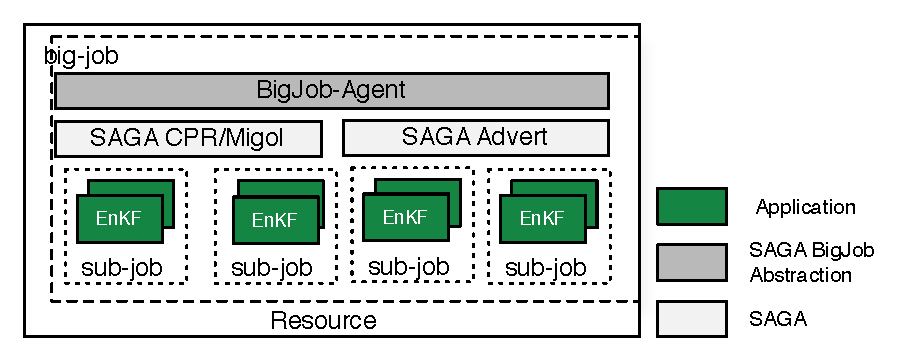
\includegraphics[width=0.44\textwidth]{./figures/enkf_bigjob.pdf}
      \caption{\footnotesize \bf stuff }
      \label{fig:abstractions}
\end{figure}

Figure~\ref{fig:abstractions} summarizes the abstractions developed
and used in this work to support the clustering of sub-jobs into a
larger big-jobs and the effective dispatching of the sub-jobs.  The
specific capability to cluster sub-jobs, is provided to the
application via the \emph{BigJob} abstraction. This abstraction
enhances the SAGA job model with the capability to allocate larger
chunks of resource for a single job.
% allocate larger chunks of resources prior to an application run.
.. A common principle to prevent this is the
usage of Glide-In jobs, which represent a placeholder for a set of
sub-tasks (see Ref.~\cite{citeulike:291860}).  For a Glide-In
job, a sufficiently large chunk of resources is requested. Smaller
sub-tasks can then rapidly be executed through the Glide-In job.
Figure~\ref{fig:remdmanager_v11} summarizes the abstractions used
within the RE framework.
\subsection{Lazarus}

% \jhanote{Need to say, what the requirements are, establish very
%   quickly why autonomics is the solution to the specific problem and
%   then talk about the solution -- first the primitive (ie scripts)
%   then the Lazarus (using BigJob and BQP).}
% \yyenote{Addressed, please have a look}  

\jhanote{Lazarus: builds upon earlier work. Integrates BigJob with BQP
  and with Fault Tolerance}

To reliably launch hundreds of reservoir simulations and collect the data
they produce repeatedly across different machines,
we needed a fast, easy to use abstraction, this lead to the use
of BigJob abstraction ~\cite{ICCS_paper, saga_royalsoc}.
After losing many jobs to various errors
such as running out of allocated diskspace, hardware failure
and file-copy failure, we quickly came to the conclusion that autonomy
and self healing are important features that we needed to incorporate 
in Lazarus to ensure all large scale history matching runs
complete successfully. With fault tolerance, we no longer wasted
thousands of SUs running simulations with missing/corrupt ensemble members.
On the other hand, the autonomy incorporated in Lazarus, while basic,
ensures that we optimize the job sizes to have a higher chance of getting
through the queue without delay and that simulations
that ran into issues or simply failed to run, are resurrected.

For the current implementation, we started off using simple, portable
python scripts -- based upon SAGA, that handles job-launching and data
migration. This makes Lazarus a modular,
scalable and extensible framework for autonomic applications based upon
the SAGA programming system.  Lazarus uses the BigJob
abstraction to launch simulations,
the SAGA file adaptor python bindings to move files from one machine
to another and BQP data from a small python wrapper around the BQP command line tool
to retrieve the optimal location and number of BigJobs required to satisfy the
computation power required.

Lazarus's healing ability depends on
user-defined tests on the data to make sure it
is not corrupt, missing, or otherwise defective. If a simulation is
found to be defective it is resubmitted to be run again. This self
resurrection ability overcomes some of the catastrophic errors
encountered when running large numbers of jobs such exceeding wall
clock time, running out of diskspace (resubmit on a different machine)
and of course node failure.

\subsubsection{Autonomy}
The Lazarus framework contains several aspects of autonomy: it has
self-configuration (deployment on resources), self optimization (using
BQP data), self monitoring (checking its own output) and of course
self healing (resubmission of faulty simulations). These aspects have
been implemented with varying level of intelligence: the self
optimization for example is a basic algorithm that uses BQP data to
assign big-jobs to resources, but does not take into consideration
bandwidth requirement and the cost of copying files across
machines. The self-healing on another hand can typically resurrect
jobs that fail due to node failure as opposed to software
failure. Many autonomic features of Lazarus will find their way into
the FAUST framework, where they will be improved to incorporate
sophisticated inherent intelligence.  

It is also worth mentioning the due to the correct programming
abstractions, we did not have to develop most of the tuning
mechanisms, but were able to write suitable interfaces to these
mechanisms.

\subsubsection{Fault Tolerance}
Lazarus has built in self-healing capabilities. These capabilities
rely on a tool-check/calibration test and output file checks. After
all simulations have finished and their output files are copied over,
Lazarus proceeds to perform a tool-check on a sane file. The purpose
of the tool-check is to make sure the tools that will be used in
checking the output files from the simulations are available and
behave according to expectations. Once the tools are verified, they
are used to check the output of all the simulations. If a simulation
is found to have missing, incomplete or otherwise faulty output, it is
flagged for resubmission.  After all output is checked, the faulty
simulations are resubmitted and upon termination, all output is
checked again. Upon success, Lazarus proceeds to the next stage.


\section{Lazarus Architecture and Application Control Flow}

\jhanote{we need to discuss in words figures 3, 4 and 5..}

\jhanote{Place in a suitable place...}  Lazarus is distinct to other
well established and successful approaches such as Accord for
autonomic computing, in that it is not a component-based programming
system but it is a framework already composed of multiple
components. Importantly the programming system that is used is SAGA --
both for the application and the Lazarus framework.

\begin{figure}
\begin{center}
%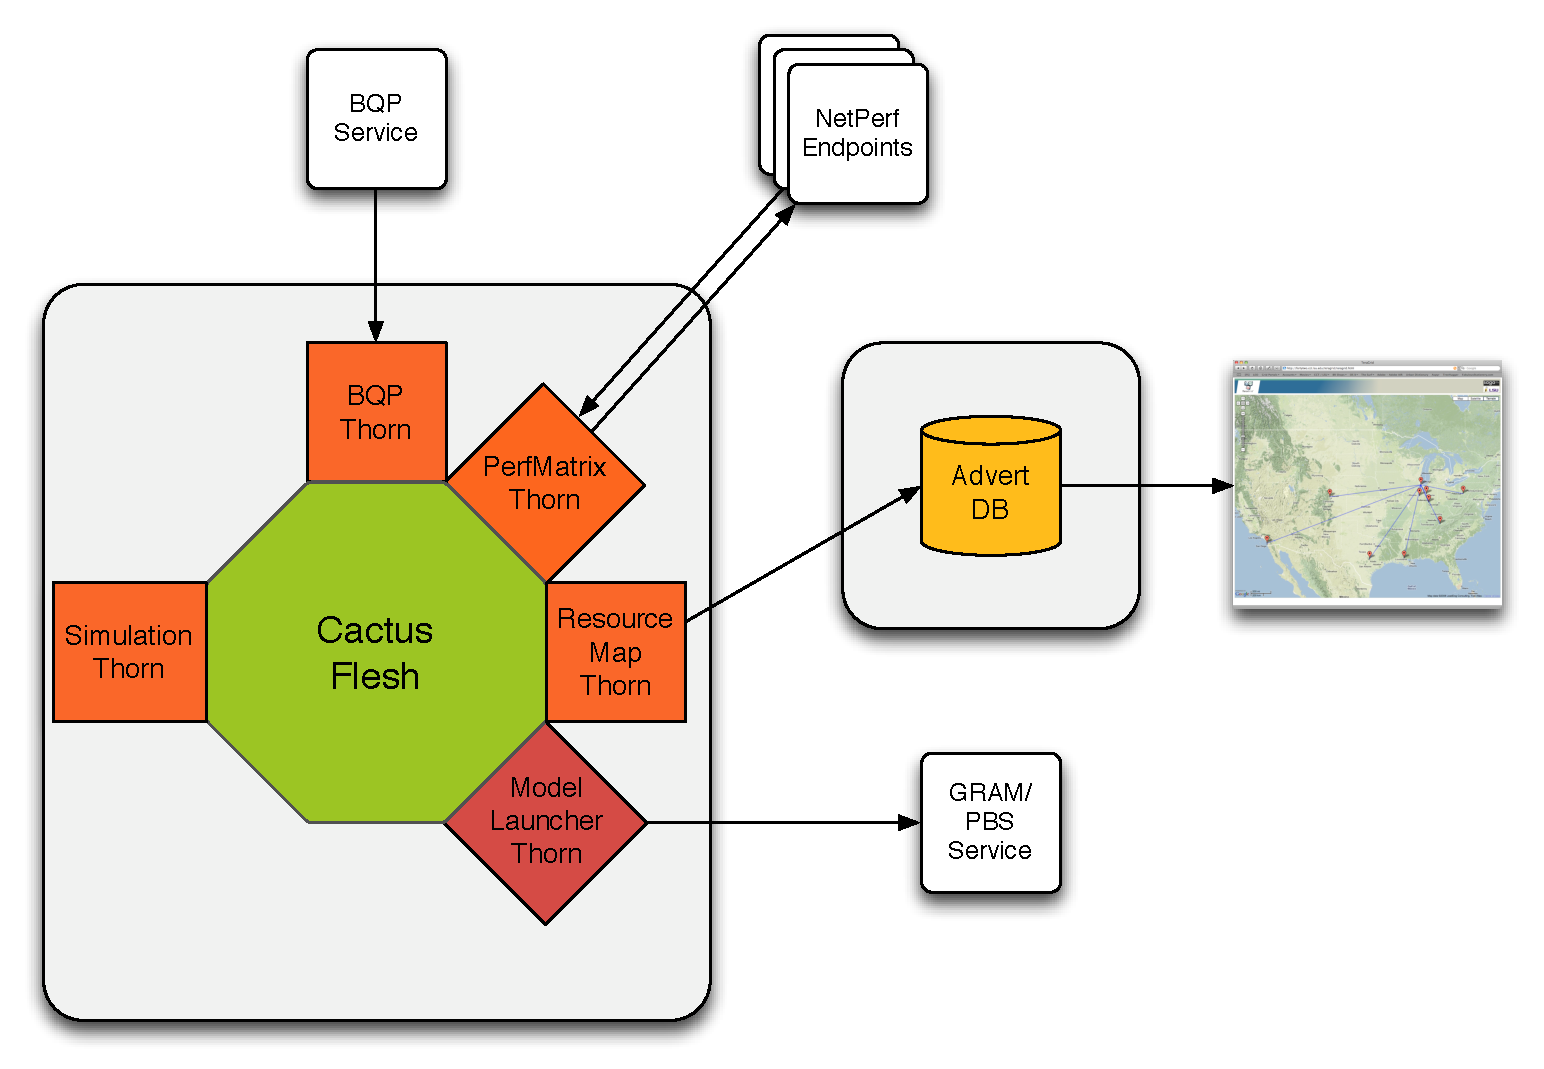
\includegraphics[scale=0.34]{./figures/ApplicationArchitecture}
%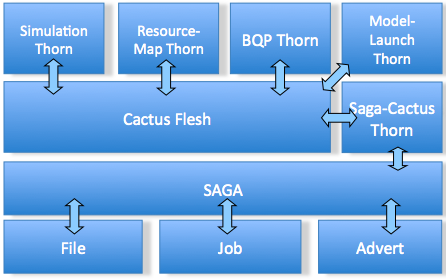
\includegraphics[scale=0.34]{./figures/kalmanfilterlayer.png}
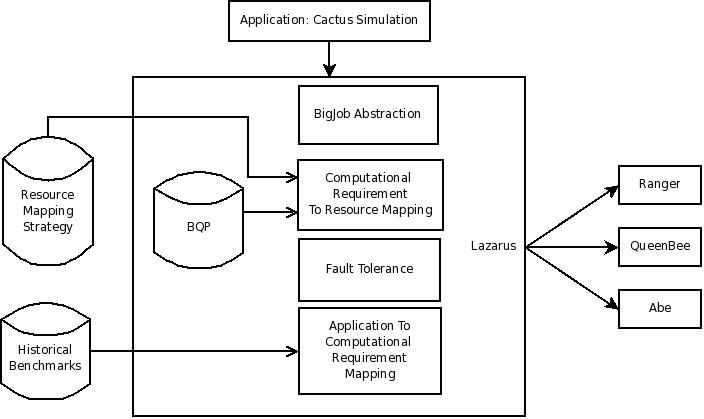
\includegraphics[scale=0.3]{./figures/Lazarus_01.jpeg}
\end{center}
\caption{\jhanote{Need to increase resolution!}  Lazarus -- An
  Autonomic framework}

\label{fig:application_architecture}
\end{figure}


\subsection{Simulation Components}
The simulation component in the Lazarus framework is based on the Cactus
framework and employs two Cactus builds: a reservoir simulation build
that uses the reservoir simulation thorns and an EnKF build that
uses the EnkF thorns. Both builds use the Cactus IO thorns and functionality
from third party libraries such as PETSc~\cite{PETSc} and HDF5.

The reservoir simulation thorn solves a system of non-linear partial differential
equations for compressible mulitphase flow through porous media. The
simulator is in effect a black-oil reservoir simulator that uses
the implicit-pressure, explicit-saturation formulation and a
finite difference discretization. The system of equations is solved
using a Krylov subspace solver using PETSc. For a prototype
implementation we chose a multiphase, multicomponent fluid flow
through porous media simulator and implemented it in the Simulation
thorn in Cactus.

The EnKF thorn is a recently implemented ensemble Kalman filter
thorn that requires, as input, the state vectors of the various
ensembles at regular intervals. These are effectively the checkpoint
files of the simulations (forecasts) in addition to their production
data. Once the EnKF has all the state vectors from all the ensembles, 
it performs the analysis and a new set of ensembles with now modified
state vectors need to be run. This process is repeated until there
are is no more historical data to match against. Typically,
production history is averaged on a monthly basis, sometimes on weekly
or even daily basis, over a period of a few years. For this reason,
a typical production run of Lazarus will involve hundreds of stages.

\subsection{Lazarus Components}

\jhanote{The following is both misleading and inelegant} s mentioned
earlier, Lazarus in its current incarnation is a set of small, fast,
portable and modular python scripts. These scripts make extensive use
of the SAGA python adaptors directly (such as the file adaptors) and
indirectly (through the BigJob abstraction).

Lazarus uses the BigJob abstraction to submit jobs to various resources.
Because the BigJob abstraction is a high-level abstraction, the user
will not need to have more knowledge than what is required to run their
application, specifically executable name, parameter file, and working directory, all of which is automated in the case of Lazarus for easier record keeping.

For runs distributed across several machines, Lazarus needs to gather
the data from all different machines into one location where the EnKF
can run. To that end, the python bindings to the SAGA file adaptors are used
to copy files over to the resource where the EnKF will run, and copied
back to all other resources after the analysis stage. Since we are not working
with a large scale production history matching run, the amount
of data transfer involved does not impose any noticeable performance issues. Naturally,
investigating the optimal location for placing the EnKF application
as discussed in \cite{escience07} will find its way into the next iteration
of Lazarus implementation and of course FAUST.

Lazarus also uses non-SAGA components, such as a small python wrapper
for BQP. This allows Lazarus, namely its resource management function, to query
BQP for the ``optimal'' job size and duration for any given resource. Lazarus
also uses a user specified check for the integrity of the simulation data. In our
case, this is done through various system and HDF5 calls to make sure the files exist,
are not sized zero, and a user specified command using HDF5 tools (h5ls) returns successfully.



\subsection{Control Flow}

\begin{figure}
\begin{center}
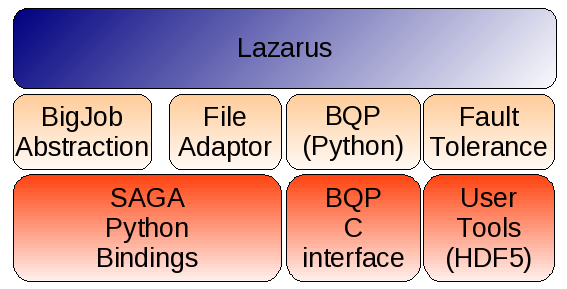
\includegraphics[scale=0.5]{./figures/Architecture.png}
\caption{Block diagrams outlining the basic structure of Lazarus. Lazarus is built on
several components: BigJob abstraction, SAGA file adaptor, BQP python wrappers and fault tolerance
functions that are based on SAGA python bindings, BQP command line tools and HDF5 tools respectively
}
\end{center}

\label{fig:application_architecture}
\end{figure}


\begin{figure}
\begin{center}
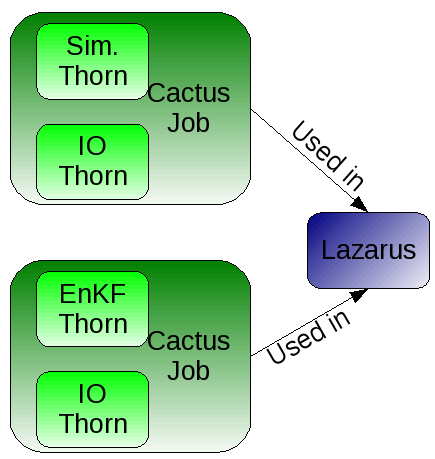
\includegraphics[scale=0.5]{./figures/Simulations.png}
\caption{Lazarus as it is being used for history matching: Cactus
built with reservoir  simulation and IO thorns for forecasting, Cactus
built with EnKF and IO thorns for analysis
}
\end{center}

\label{fig:application_usage}
\end{figure}


\begin{figure}
\begin{center}
 %  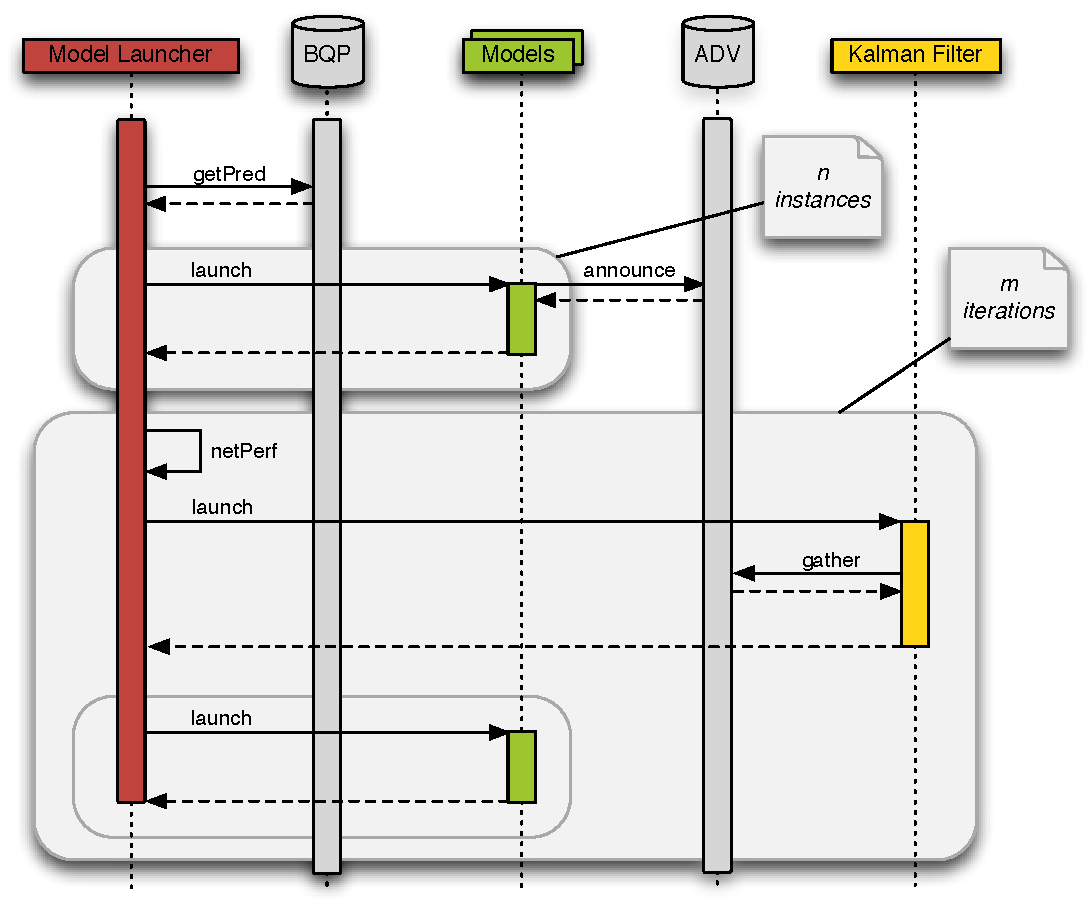
\includegraphics[scale=0.5]{./figures/SequenceDiagram}
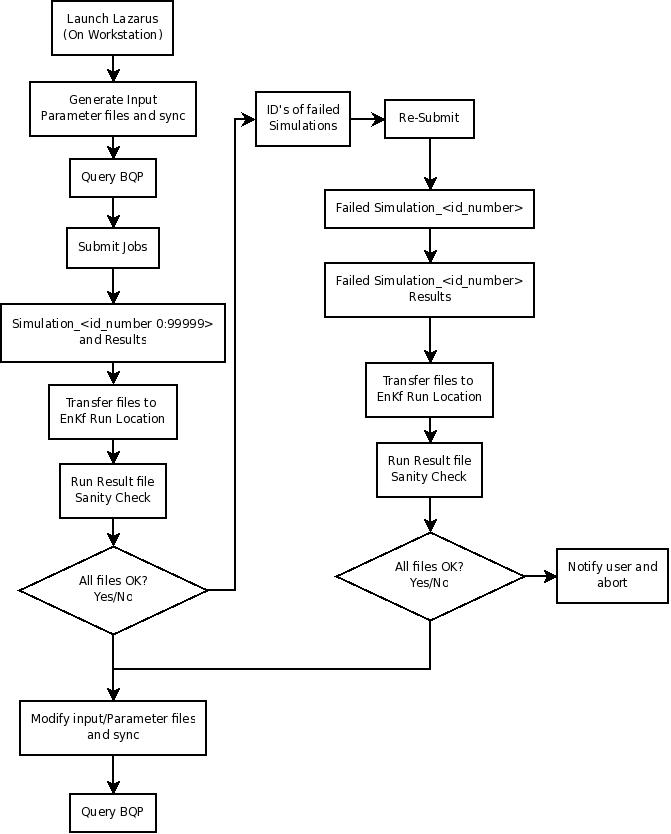
\includegraphics[scale=0.35]{./figures/Diagram1.jpeg}
\end{center}
\caption{A high-level
  overview of the control flow in Lazarus}
\label{fig:controlflow}
\end{figure}

%The application starts by getting BQP data for a list of candidate
%machines, assigns simulations to machines and submits the jobs to the
%respective machine scheduler. Once all the simulations are submitted,
%the history matching application (in our case a Kalman filter) is
%submitted to run. The Kalman filter application is run on the
%machine that will run 50\% or more of the entire simulations or the
%machine that has the highest bandwidth amongst the machines used for
%the simulations.  Once the simulations start, they notify the advert
%service of their starting time and location; upon successful
%completion, they also notify the advert service of the path of the
%files they output.  Meanwhile the history matching application is
%notified of the completion of the simulations and modifies the models
%used in the reservoir simulation. The modified models are then
%submitted again as a second stage and the entire processes is
%repeated.

These points need to be made clear in this sub-section? \newline
 {\it Mapping of physical-model
  requirements into compute-resource requirements} \newline {\it
  Mapping compute-resource requirements into available
  resources}\newline


To prepare for launching Lazarus, a model generator is required to create
the initial data (initial state vectors) for all the ensembles. This is typically
done a priori to running Lazarus, and performed on one resource then synchronized
against all others to ensure consistency.

Before launching Lazarus, some input parameters need to be specified.
These are the executable names, working root directory, simulation directories,
number of simulations per stage, number of stages and so on. Given 
the number of jobs per stage, and historical benchmark information on various
machines, an estimate for the total SUs required is sent to the Lazarus
resource manager. The resource manager queries BQP for the optimal sizes and durations
and creates a list of BigJobs, their sizes, durations and the resource/queue
where they will be submitted. If we have more than one resource available, the SU
requirement is satisfied based on a round-robin algorithm, iterating over
resources and adding BigJobs until no more BigJobs need to be submitted.

Once the resource list is formulated, Lazarus uses the BigJob abstraction to submit
jobs to all BigJobs in the resource list. The status of the jobs and BigJobs
is reported on regular intervals through a logging mechanism. Upon completion
of all the subjobs, Lazarus performs a calibration test where it runs
the user-specified output-check on a pre-validated file, to ensure all the tools
are in place and in working order. It then proceeds to check the output from all simulations to ensure sanity of output. Simulations that have faulty output are then
collected into a list and resubmitted. The output is again checked for sanity: if
all is well we proceed with the EnKF run (i.e. the analysis) and if not
Lazarus will abort with a detailed log file of the error. This is mainly to safeguard
against wasting SUs on corrupt runs. Once the analysis is complete,
Lazarus repeats the forecast iteration with the newly modified state vectors and
the history matching continues.



\section{Failure Modes}

% \jhanote{Which failure modes are relevant here? Remove those that are
%   not}\yyenote{Fixed}
As early as the first non-trivial Lazarus run we encountered failures. They
varied in nature (hardware/environment) and severity. As Lazarus progressively
used more resources, many more failure modes were encountered.
Many were errors that are irrecoverable and resulted in a
cold restart from scratch; others were recoverable with a simple simulation 
result-check fault tolerant component built into Lazarus.

Hardware failure:
\begin{itemize}
\item{Lost a compute node from the pool}
\item{Lost a network connection to a machine, BQP or the advert service}
\item{Could not write to /scratch because it was taken down for maintenance}
\end{itemize}
From all of these modes of failure, we found that we reliably recover
from node failure and failure to write data to disk, but not network failure. The
status of any given job is reported in a one-way poll for current state. This
has obvious limitations so we will also be using the "heart-beat" monitor in FAUST
once it is available.

Software environment failures:
\begin{itemize}
\item{Missing or wrong shared libraries}
\item{Wrong or inadequate environment variables}
\item{Run out of quota on disk, wrote too many files to the same directory}
\item{Run out of SU's in the allocation}
\item{No internet connection to the compute nodes (no BQP, no advert service)}
\item{MPI error that causes a simulation to stall (this happened because of a faulty installation and was corrected)}
\end{itemize}
In software environment failures, typically jobs terminate with errors or 
are killed, before the simulations results are written to disk. Unsurprisingly we ran
into all of these failures while developing Lazarus, and were able
to recover from all of them except for the network connectivity in the compute
nodes, as this would register the job's state as "unknown". This would be solved
with the aforementioned heart-beat monitoring system in FAUST.

Actual simulation failures:
\begin{itemize}
\item{Missing parameter files or executable}
\item{Wrong parameter files, or erroneous setup of parameter files}
\item{Divergence in the solver, causing NaN shuffling and leading to exceeding the requested wall clock time}
\item{Under-estimation of the required wall clock time}
\item{Hitting /scratch or /home too often (because of checkpointing), leading to very low access speeds and exceeding the requested wall clock time}
\end{itemize}
Some of the simulation failures are relatively easy to guard against,
namely the wrong parameter file or missing executable. The other errors
however are harder to detect and rectify.

\subsection{Needs to be Moved}
One of the recent improvements in deployment is the use of the python
bindings to the SAGA-based BigJob abstraction % \yyenote{I think the
%   name here should change as this is not really FAUST yet but loosely
%   labelled FAUST}. \jhanote{Yes, I agree. Dunnit} 
Using these scripts, a user-specified number of stages each containing
a user-defined number of models can be launched to the grid. As the
models of a given stage run to completion, a second set of
error-checking jobs are launched that ensure all the models ran to
completion before the Kalman gain calculation is performed. This
error-checking mechanism attempts to re-submit the failed jobs, and if
met with failure a second time, the stage is halted to allow for user
intervention. \yyenote{that is what I am implementing at the moment}

\jhanote{Mapping: Need discussion on the two-levels of decision
  making. I thought we had done this!}

\jhanote{The latter could be done via BigJob Abstraction or without
  (statically map to an available resource, with or without the aid of
  BQP).  The advantage of BigJob abstraction (and ultimately FAUST) is
  the flexibility it provides -- wanna call is late binding? or
  loose-coupling..  call it what you may.}

\jhanote{there is the following blurb from the ICCS paper which we
  should either incorporate or acknowledge} We have developed a
mechanism whereby EnKF can be solved using multiple-resources, using
application-level scheduling applied dynamically~\cite{saga_tg08}, ie
mapping the sub-tasks requirement to the resources available at the
instant the sub-tasks become available and ready to run, as opposed to
{\it a priori} static method of job submission.  For the problem size
studied, the sub-tasks required mostly less than 32 processors. For
this paper we used the earlier developed frameworks and deployed it on
a single large machine -- NCSA's Abe. A mechanism (multiple,
distributed versus single machine) that is more efficient for physical
models with sub-tasks that have typically low processor counts, will
not necessarily be the more efficient as the typical sub-task size
increases. Therefore it is crucial that any general-purpose solution
be usable on both single large machines to multiple machines.  We can
enhance throughput further by applying the Glide-In mechanisms
discussed in the earlier section, which facilitate dynamic tasks being
aggregated from similar sub-tasks. We will report on the results of
this and whether the framework can be used on high-end petascale
supercomputers in future work.


\section{Experiments: Results and Discussion}

In this section, we discuss the Experiments we performed, but first
we discuss the design of the experiments.

As alluded to Grids are dynamic and in principle provide an effective
infrastructure for applications with dynamic resource requirements, as
well as hard-to-predict resources. The underlying motivation for these
experiments is to first establish that the Lazarus framework enables
the effective utilization of Grid resources. The second, design
decision for experiments is to determine if autonomic behaviour -- in
this case, the ability to use system-level information to decide which
resources to use dynamically, as opposed to the manual
intervention/decision, can lead to performance gains.

% \jhanote{Yaakoub, please put in a paragraph about the workload}
% \yyenote{Done}

The workload is defined as reduced version of a typical history
matching run. We start with an ensemble of one hundred members and we
need to perform five analysis/Kalman-filter runs. Since this sample
workload is representative of the size of a typical large history
matching run and a reduced form of its duration, any consistent
reduction in the total time to completion will eventually have a
larger impact on larger runs with more stages.

We define the \tc as the time in seconds it takes to complete the
workload. There are several components to the \tc. First, is the time
that it takes to submit to the queuing system, file-transfer (in and
out). In a way this is overhead, and we label this as $t_{overhead}$.
The second component is the time that the submitted jobs wait in queue
for resources requested to become available. We label this as
$t_{wait}$; the final component is the time the runtime that
simulations actually take to complete, which we label as
$t_{run}$. Thus: \tc = $t_{overhead}$ + $t_{wait}$ + $t_{run}$.

In the first stage of experiments, we determine the \tc for a single
TG machine, but repeat the experiment for different TG machines and
repeat 4-5 times at different times of the week, so as to get
uncorrelated data.  This provides a measure of base-line performance.

We then, repeat experiments using more than one computational resource
on the TG. To be precise, we employ more than one computational
resource towards the solution of a single instance of the problem.
Given that are experiments are capable of utilizing three different TG
resources, using two-resources at a time, gives us three different
combinations. As the results from the single-resource configuration
show, the individual resources have somewhat different intrinsic
performance, which should be factored when taking into account the
combined performance. As a logical extension, we perform an experiment
wherein we utilize all three different TG resources.  An important
result, that holds in general, but also for the specific instances
investigated here, is that on average, as the number of resources
increases the \tc to solution decreases. This is evidenced from the
fact \tc for (R,Q) is lower than \tc (R) or \tc (Q). The large error
bars are due to the fluctuations in the waiting times; it is important
to point out that the $t_{run}$ decreases, but the overall number of
CPU hours utilized does not increase. This is a reconfirmation of
the use of higher-level abstractions for enhanced performance.

In the final experiment, we utilize a type of information service --
BQP (for queue prediction) and incorporate it into the Lazarus
framework and make use of it through autonomic behaviour.  As the
right most datapoint shows, the utilization of BQP to determine which
resources and which configuration are used leads to a drastic
reduction in \tc compared to the simple case where Lazarus framework
was used without autonomic behaviour. This is a very powerful
demonstration of the fact that autonomic behaviour -- however
elementary, can lead to significantly improved performance.

\begin{itemize}
\item Define workload.
\item Determine  \tc when using 1 machine 
\item Determine \tc when using same machine over 5 day average i.e. repeat 5    times, at least 3 times
\item Determine \tc when scaling up to 2 machines, 3 machines 
\item point out fluctuation in work-load and response time
\item point out that the experiment was repeated 4 times for non-BQP
  cases and repeated 3 for the BQP case (with experiment ongoing on
  the 4th experiment).
\end{itemize}

\begin{figure}
\begin{center}
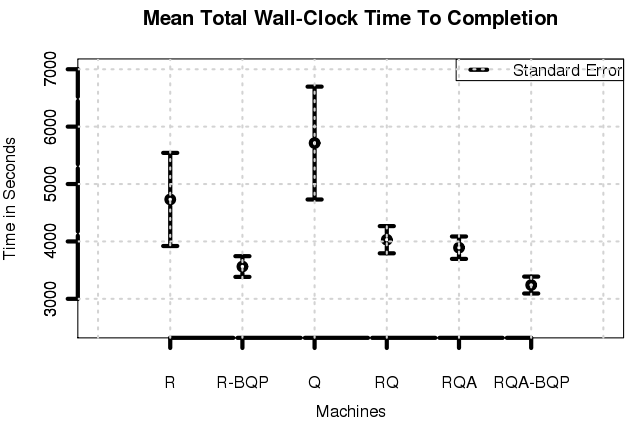
\includegraphics[scale=0.35]{./figures/Figure7.png}
\end{center}
\caption{From Left to Right: (i) Ranger, (ii) Queen Bee,
  (iii)Ranger+QueenBee, (iv) Ranger+QB+Abe, (v) BQP-All
  Machines. \jhanote{ Need to refine... Need higher resolution graph!!}}
\label{fig:application_architecture}
\end{figure}

\begin{table}
\begin{tabular}{|c|c|c|c|c|}
\hline Sample \# & Machine & Queue & Num. Cores & Duration (hrs) \\ 
\hline 1 & Ranger & normal & 64 & 2:00 \\ 
\hline 1 & Ranger-BQP & development & 128 & 1:00 \\ 
\hline 
\end{tabular} 
\caption{A table with the results for Ranger with and without BQP. While the
    total number of SUs consumed remains constant, the queue, size and duration
    of the BigJob changes}
\end{table}


\begin{table}
\begin{tabular}{|c|c|c|c|c|}
\hline Sample \# & Machine & Queue & Num. Cores & Duration (hrs) \\ 
\hline 1-3 & Ranger & development & 64 & 1:30 \\ 
\hline 1-3 & QueenBee & checkpt & 128 & 2:00 \\ 
\hline 1-3 & Abe & dque & 64 & 2:00 \\ 
\hline 4 & Ranger & development & 64 & 2:00 \\ 
\hline 4 & QueenBee & checkpt & 16 & 1:00 \\ 
\hline 4 & Abe & dque & 64 & 1:00 \\ 
\hline 
\end{tabular} 
\caption{A table with the results of the resources used and in
  the configuration of the resources -- as determined, by the
  number of cores, duration and queue. The decision on
  resource and resource configuration is aided by BQP -- which 
  makes a locally optimal decision. \jhanote{we need to repeat
    this experiment a few times; based upon the outcome we should either
    mention that BQP always gives us this configuration, or hopefully we
    can say that BQP selects differently}}
\end{table}

\jhanote{Did we get data for sample 4? was it different?}

\jhanote{In Table I, can you also elaborate the results of i) num cores and
ii) duration chosen for the Ranger only BQP submission.}



\section{Challenges and Discussion}

\begin{itemize}
\item Talk about the fixed granularity of BQP and the problems that this
engenders
\item Talk about fault-tolerance
\item Talk about how different machines have different queuing policies
  and how an autonomic system like Lazarus can ``probe'' the queuing
  system to understand the non-public policy and adapt irrespective.
\end{itemize}

% \jhanote{What are the fault-tolerance issues that are encountered?
%   How do we solve them? How could they be solved by using SAGA-CPR
%   (just sketch out changes that need to be undertaken)}

% \jhanote{need to reference prior work done by Manish on autonomics and
%   on oil reservoir in particular. What makes our work different?  Can
%   the two converge? SAGA-Accord?}
% \yyenote{Yes and no, physics and problems we are solving are different, 
% but yes we can converge. I would not say interchangeable, because well 
% optimization studies do not require a global sync like we have in the EnKF
% Added stuff in the intro about Manish, hope he likes it}  

The advantages of constantly running jobs on machines is the
development of an intuition to the state of the machine through
constant use. This is quantified in confidence numbers from
BQP. Interestingly enough, we could discern a higher chance of running
before deadlines during weekends than weekdays, and how some machines
favor larger jobs that have short durations and how other machines
favor the opposite.

A major issue in our use of the BQP is the confidence and quantile
numbers. A detailed analysis is required to better quantify what those
numbers mean when submitting many BigJobs across different machines,
and how the choice of confidence and quantile ultimately affect the
total wall clock time to completion. \jhanote{needs explaination}

Since we collected data from BQP without knowing it's granularity, we
tend to oversample the data to avoid undersampling and obtaining a
misrepresentative view.  This obviously leads to a small (order of
minutes) computational cost but is an issue that needs to be
addressed. \jhanote{what is oversampling? why is it misrepresentative?
  please elaborate}

Perhaps the biggest challenge we encountered, and most frustrating,
was failure that went undetected, and lead us to waste SUs, hours in
the queue and of course hours waiting for results that were
corrupt. Many of these modes of failure can be solved using a
heart-beat from the actual simulation to a monitoring service that
allows the simulation to register its current state, current
iteration, progress rate, state of data, convergence data from the
solver etc... This will be implemented using the SAGA C++ API in
Cactus as a heartbeat thorn, and the monitoring service will be
implemented as a functionality in FAUST.  \jhanote{Similar failures,
  but different machines and different solutions. Therefore need to
  make the case for FT service i.e., generalise FT}


\section{Future Work and Conclusion}

\jhanote{Talk about forward and reverse scheduling/resource
  reservation: normally we define a workload/requirement, and then map
  that to the best available resource. Reverse scheduling is, find the
  best resource/resource configuration and then adapt the workload to
  the best resource/resource configuration. BQP based autonomics,
  enables this to happen}

\jhanote{Need a paragraph about how BQP based Autonomics can be used
  in additional ways (possibly)? Set the case for grid2009/faust..}

One of the planned extensions to Lazarus is the addition of adaptive
queuing systems. As it stands, Lazarus will submit optimized BigJobs to
resources and wait for them to get through the queue, run and terminate.
 When the number and size of subjobs is
sufficiently large and the resources considerably congested,
this will be a considerable amount of time
during which larger, less congested resources may have come online or better BQP
BigJob configurations have emerged; all of this
while the original BigJobs have not started to run. A BigJob can then be scheduled
on a new resource or another BigJob of different size and duration
can be submitted to the queue and existing BigJobs that are in the queue
can be deleted. This adaptive ability in Lazarus will be implemented
in a rudimentary level using python scripts, SAGA-python bindings and of
course BQP interfaces; however a more robust, service based implementation
will be part of the FAUST framework.

In this paper we have demonstrated the very first beginnings of the
SAGA-based framework (Lazarus) that can be utilized by a broad range
of different applications to utilize Grids for autonomic computing.
Lazarus is distinct to other well established and successful
approaches such as Accord for autonomic computing, in that it is not a
component-based programming system but it is a framework already
composed of multiple components. Importantly the programming system
that is used is SAGA -- both for the application and the Lazarus
framework.

\jhanote{some points to elaborate in the discussion}

\begin{itemize}
\item Lazarus will evolve to utilize more sophisticated Information Services.
\item Lazarus in of itself will utilize other frameworks (e.g., FAUST)
\jhanote{Need to make connection, or announce the arrival of FAUST}
\item Lazarus and its uptake by other applications.
\end{itemize}


% We created a single set of Globus adaptors and deployed them on
% distinct Grids. Our application successfully utilized these
% adaptors, without any further customization, which goes to show that

%We also discussed how the deployment of this model application across
%two distinct Grids was trivial as it only required the deployment of
%of the appropriate SAGA adaptors.  



% There are many applications that need to use federated
% Grids~\cite{clade06, gin_paper}.  Utilizing SAGA to develop, or at
% least provide Grid-functionality is a useful strategy. Therefore, if
% the development and deployment of applications across federated grids
% is to be facilitated, SAGA adaptor activity -- development and
% deployment, needs to be self-sustaining and thus requires explicit
% support, from both the middleware developers and resource providers.

% The success of e-Science critically depends upon the availability of
% e-Infrastructure.  But the promise of e-Science will be hollow without
% delivery of the applications and application-enabling paradigms and
% technology that can effectively utilize this new infrastructure. We
% believe SAGA is an important first step in this direction.

\section{Acknowledgments}
We acknowledge Andre Luckow, who should have been an author on this
paper, had it not been for bureaucratic hurdles.  SJ acknowledges UK
EPSRC grant number GR/D0766171/1 for supporting SAGA and the e-Science
Institute, Edinburgh for the research theme, ``Distributed Programming
Abstractions''.  SJ also acknowledges financial support from
NSF-Cybertools and NIH-INBRE Grants. YE acknowledges the Department of
Energy and Louisiana Board of Regents (award No. DE-FG02- 04ER46136)
for providing funding and support. YE would like to acknowledge
Prof. Chris White, Prof. Mayank Tyagi and Dr. Xin Li. This work would
not have been possible without the efforts and support of other
members of the SAGA team. The authors acknowledge the Texas Advanced
Computing Center (TACC) at The University of Texas at Austin, LONI and
NCSA for providing HPC resources that have contributed to the research
results reported within this paper. This work has been made possible
thanks to the internal resources of the Center for Computation \&
Technology (CCT) at Louisiana State University.

\bibliographystyle{IEEEtran} 
\bibliography{saga_tg08}
\end{document}

Another abstraction
-- the SAGA Glide-In abstraction is used to support the commonly
occurring requirement to schedule multiple sub-tasks relative to each
other and not in competition with other jobs submitted to the batch
queue system.  Thus, a \texttt{big\_job} and \texttt{sub\_job} object
are defined; for each \texttt{big\_job} object, a Glide-In job with
the desired number of resources is started, and \texttt{sub\_job}
objects -- which correspond to individual replicas, are mapped to a
\texttt{big\_job} using the jobid as reference. It is helpful to
reiterate that although there is a big\_job object, it is submitted
as a Glide-In job, and that BigJob abstraction in turn utilises the
Glide-In abstraction to map the individual big-job and sub-jobs to
physical resources.

Figure~\ref{fig:abstractions} summarizes the abstractions developed
and used in this work to support the clustering of sub-jobs into a
larger big-jobs and the effective dispatching of the sub-jobs.  The
specific capability to cluster sub-jobs, is provided to the
application via the \emph{BigJob} abstraction. This abstraction
enhances the SAGA job model \jhanote{Need a sentence or two about what
  ``enhancing the SAGA job model'' means, ie in turn outlining what
  the SAGA Job Model is?}  with the capability to allocate
larger chunks of resource for a single job.
% allocate larger chunks of resources prior to an application run.
\jhanote{AndreL: Not sure what the commented out line was about.. if
  you'd like to reinstate, please clarify/elaborate}
